\section{Case Study}\label{sec:case-study}

\subsection{Case Study Design}

In order to identify the architectural differences between implementations of microservice architectures implemented with REST and GraphQL interfaces, a case study is performed.
To be independent of past design decisions, the case study is performed on a newly implemented example project.

The example project implements the setting of an online shop as shown in \autoref{fig:cs-setting}.
The shop keeps its inventory in one or more warehouses.
When the user orders items from the shop, the inventory is checked and the ordered items are reserved.
When the user's bank processes the payment to the shop, the reserved items of the order are shipped to the user.
For this case study, the user's payment instruction to their bank, and the bank's processing of the payment is outside of the scope.

\begin{figure}[!htb]
    \centering
    \begin{tikzpicture}[
    node distance=3cm,
    comp/.style = {
        draw,
        circle,
        text width = 2cm,
        align = center,
        thick
    },
    l/.style = {
        text width = 3cm
    }
]

\node[comp] (user) {User};
\node[comp, rectangle, right=of user] (shop) {Shop};
\node[comp, rectangle, right=of shop] (ware) {Warehouse};
\node[comp, rectangle, below=of user] (bank) {Bank};
\node[comp, rectangle, below=of ware] (post) {Postal Service};

\draw[->, thick] (user) -- node[above, l, align=center] {orders items} (shop);
\draw[->, thick] (user) -- node[right, l, yshift=.5cm] {instructs payment} (bank);

\draw[->, thick] (shop) -- node[above, l, align=center] {checks inventory \& reserves items} (ware);
\draw[->, thick] (shop) -- node[right, l] {ships items} (post);

\draw[->, thick] (bank) -- node[right, l] {sends payment} (shop);

\draw[dashed] ($(user)!0.5!(shop)$) + (0, 1cm) -- +(0, -5cm);

\end{tikzpicture}
    \caption{Setting of the Case-Study}\label{fig:cs-setting}
\end{figure}

In the first step of the case study, this setting is implemented twice with a microservice architecture, first using \ac{REST} and then using GraphQL.% checktex 13
After implementing the case study, the architecture of both implementations is compared.
At this point, a service cut was intentionally not defined to evaluate if the different technologies also suit a different service cut.

Using both implementations of this scenario, the performance can be compared.
This can be done by defining a set of request scenarios (e.g.~a user orders 5 items and pays immediately afterward).
The resulting load on the system can then be measured in two different ways.
First, the average response time until a user's request is executed can be measured.
This is important as fast processing of requests is essential to a user's experience of using the system.
Second, the generated load on the internal network connecting the microservices can be measured.
While this case study only utilizes a single network, for geographically distributed microservices, the network can be a bottleneck.

The last part of the case study is to evaluate a schema evolution of the data held by the microservices.
This step consists of introducing the additional constraint, that the shipping cost of an order is now dependant on the weight of the items.
This means, that each item now has an additional property, which is consumed within the system.

\subsection{Implementation of \acs{REST} Microservices}

To implement the case study using a \ac{REST} \ac{API} for communication between the microservices, a service cut consisting of four different services was chosen.

\paragraph{Inventory Service}

The inventory service manages the available \textit{items}, and where they are stored.
It maintains a set of \textit{warehouses} where items are located.
Items and warehouses are associated with each other by \textit{stock positions}.
While the items themselves maintain only information such as name or price, stock positions maintain how many of one item is stored in a warehouse.
Additionally, each stock position stores how many of an item in the warehouse is available.
In this case, an item is available, if it is not yet part of an existing order.

\paragraph{Order Service}

The order service accepts the user's \textit{orders}.
When a new order is created, the service first verifies that for each \textit{position of the order} enough items are in stock to fulfill the order.
This is done by requesting the stock positions of the items from the inventory service.
If enough items are available, the items are reserved (marked as unavailable).
Next, the shipping service is contacted to calculate the shipping cost for the order and to create a new shipment.
The total of the order is calculated and the payment service is instructed to create a payment with the calculated sum.
The order service is the main service, users interact with.
Apart from that, it provides endpoints to the other services to update the status of the order (i.e. \textit{payment received} or \textit{shipped}).

\paragraph{Shipping Service}

The shipping service manages \textit{shipments} for orders.
In this case study, it only calculates the cost of shipping for an order.
In a real-world implementation, this service could additionally interface with third-party \acp{API} of postal services and print labels for the packages.

\paragraph{Payment Service}

The payment service manages \textit{payments} for orders.
Similarly to the shipping service, this service only stores the due amount, but could interface with payment processors in a real-world setting.


A complete overview of the interaction of the services is shown in \autoref{fig:interaction}.
The user creates a new order~\raisebox{.5pt}{\textcircled{\raisebox{-.9pt} {1}}}, the order service checks if enough items are in stock~\raisebox{.5pt}{\textcircled{\raisebox{-.9pt} {2}}} and reserves the items if they are~\raisebox{.5pt}{\textcircled{\raisebox{-.9pt} {3}}}.
Then, a new shipment is created by the shipping service~\raisebox{.5pt}{\textcircled{\raisebox{-.9pt} {4}}} and a new payment is created by the payment service~\raisebox{.5pt}{\textcircled{\raisebox{-.9pt} {5}}}.
When the payment is received~\raisebox{.5pt}{\textcircled{\raisebox{-.9pt} {6}}}, the order is updated~\raisebox{.5pt}{\textcircled{\raisebox{-.9pt} {7}}} and the shipping service is instructed to ship it~\raisebox{.5pt}{\textcircled{\raisebox{-.9pt} {8}}}.
Finally, the items are booked out from the inventory~\raisebox{.5pt}{\textcircled{\raisebox{-.9pt} {9}}}.

\begin{figure}[!htb]
    \centering
    \begin{tikzpicture}[
    node distance=3cm,
    comp/.style = {
        draw,
        circle,
        text width = 2cm,
        align = center,
        thick
    },
    l/.style = {
        text width = 3cm
    }
]

\node[comp, color=theme5, fill=theme5!10!white] (order) {Order Service};
\node[comp, below=of order, color=theme1, fill=theme1!10!white] (payment) {Payment Service};
\node[comp, above=of order, color=theme3, fill=theme3!10!white] (inventory) {Inventory Service};
\node[comp, right=of order, color=theme2, fill=theme2!10!white] (shipping) {Shipping Service};

\node[comp, left=of order] (client) {Client};
\node[comp, left=of payment] (paymentProcessor) {Payment Processor};

\draw[->, thick] (client) -- node[l, above, align=center] {\raisebox{.5pt}{\textcircled{\raisebox{-.9pt} {1}}} create order} (order);
\draw[->, thick] (order) to [bend left] node[l, left, align=right] {\raisebox{.5pt}{\textcircled{\raisebox{-.9pt} {2}}} check stock} (inventory);
\draw[->, thick] (order) to [bend right] node[l, right, align=left] {\raisebox{.5pt}{\textcircled{\raisebox{-.9pt} {3}}} reserve item} (inventory);
\draw[->, thick] (order) to [bend left] node[l, above, align=center] {\raisebox{.5pt}{\textcircled{\raisebox{-.9pt} {4}}} create shipment} (shipping);
\draw[->, thick] (order) to [bend right] node[l, left, align=right] {\raisebox{.5pt}{\textcircled{\raisebox{-.9pt} {5}}} create payment} (payment);
\draw[->, thick] (paymentProcessor) -- node[l, above, align=center] {\raisebox{.5pt}{\textcircled{\raisebox{-.9pt} {6}}} payment information} (payment);
\draw[->, thick] (payment) to [bend right] node[l, right, align=left] {\raisebox{.5pt}{\textcircled{\raisebox{-.9pt} {7}}} update order} (order);
\draw[->, thick] (order) to [bend right] node[l, below, align=center] {\raisebox{.5pt}{\textcircled{\raisebox{-.9pt} {8}}} ship order} (shipping);
\draw[->, thick] (shipping) to [bend right] node[l, right, align=left, text width=3.2cm] {\raisebox{.5pt}{\textcircled{\raisebox{-.9pt} {9}}} book out items} (inventory);

\end{tikzpicture}
    \caption{Service Interactions}\label{fig:interaction}
\end{figure}

\subsubsection{Technology Stack}

Each \acs{REST} microservice was implemented using the general-purpose programming language Java, and the Spring framework\footnote{\url{https://spring.io}}.
Findings of Schermann~\cite{Schermann2015} show, that Java is the most commonly used programming language for microservices.
Spring is a widely used framework for enterprise applications.
According to Snyk's annual \acs{JVM} Ecosystem Report~\cite{Vermeer2020}, 6 out of 10 \acs{JVM} developers use the Spring framework.
Spring is a modular, open-source framework consisting of a set of libraries providing for example dependency injection, data access, a server-side web framework, or cloud integration.

Each of the services is packaged as a Docker\footnote{\url{https://www.docker.com/}} Linux container.
These containers allow to easily distribute the packaged service and simplify the creation of replicas.
The containers for the microservices expose a port to accept \ac{HTTP} requests, that will be handled by the Spring framework.
However, each container is assigned its own IP address, which makes scaling difficult, as the destination for requests needs to be known beforehand.
Thus, an additional container running Traefik is placed before the microservice containers.
Traefik\footnote{\url{https://containo.us/traefik/}} is a reverse proxy and load balancer designed for microservices and has various integrations with different kinds of infrastructure, such as Docker or Kubernetes.

The microservices use the PostgreSQL\footnote{\url{https://www.postgresql.org/}} database system for data storage.
However, multiple instances of the same microservice share just one instance of a containerized database.
In a real-world deployment, the database should not be containerized at all, but rather a distributed database cluster should be used, to achieve high availability, redundancy, and high performance.
Communication with the database is implemented using the Spring Data \acs{JPA}, which provides convenient access to \ac{JPA} data sources.

\begin{figure}[!htb]
    \centering
    \begin{tikzpicture}[
    node distance=1.25cm,
    container/.style = {
        draw
    },
    application/.style = {
        draw,
        regular polygon,
        regular polygon sides = 4,
        text width=.5cm,
        align = center
    },
    database/.style = {
        draw,
        cylinder,
        shape border rotate=90,
        aspect=0.25,
        text width = .5cm,
        minimum height = 1cm,
        align = center%,
        %cylinder uses custom fill, cylinder body fill=white, cylinder end fill=black!5
    },
]

\node[draw, text width=3cm, align=center, minimum height=1cm] (traefik) {
\includegraphics[width=.5cm,page=1]{images/image.pdf}\\ Reverse Proxy};

\draw[->] ($(traefik)+(0,1.5cm)$) -- node[above,yshift=.25cm,text width=5cm,align=center] {\acs{HTTP} requests\\(external and internal)} (traefik);

\node[application, color=theme5, fill=theme5!10!white, below=1.5cm of traefik] (order1) {O};
\node[application, color=theme5, fill=theme5!10!white, left=of order1] (order2) {O};
\node[application, color=theme3, fill=theme3!10!white, left=of order2] (inventory) {I};
\node[application, color=theme1, fill=theme1!10!white, right=of order1] (payment) {P};
\node[application, color=theme2, fill=theme2!10!white, right=of payment] (shipping) {S};

\draw[->] (traefik) -| node[right, yshift=-1cm] {\footnotesize\texttt{/inventory/*}} (inventory);
\draw[->] (traefik) -- (order1);
\draw[->] (traefik) -- ($(traefik)!0.5!(order1)$) -| node[above, xshift=1.25cm] {\footnotesize\texttt{/order/*}} (order2);
\draw[->] (traefik) -| node[right, yshift=-1cm] {\footnotesize\texttt{/payment/*}} (payment);
\draw[->] (traefik) -| node[right, yshift=-1cm] {\footnotesize\texttt{/shipping/*}} (shipping);

\node[database, color=theme3, fill=theme3!10!white, below=of inventory] (invDb) {};
\node[database, color=theme1, fill=theme1!10!white, below=of payment] (payDb) {};
\node[database, color=theme2, fill=theme2!10!white, below=of shipping] (shipDb) {};
\node[database, color=theme5, fill=theme5!10!white, below=of $(order1.south)!0.5!(order2.south)$] (ordDb) {};

\draw[->] (inventory) -- (invDb);
\draw[->] (order1) |- (ordDb);
\draw[->] (order2) |- (ordDb);
\draw[->] (payment) -- (payDb);
\draw[->] (shipping) -- (shipDb);

\end{tikzpicture}
    \caption{Containers for the \acs{REST} Microservice Architecture}\label{fig:rest-containers}
\end{figure}

A deployment with two Order microservices is shown exemplary in \autoref{fig:rest-containers}.
Traefik accepts all \ac{HTTP} requests --- regardless whether they come directly from users, or other microservices --- and routes them to the appropriate microservice depending on the so-called context path.
The context path specifies a path prefix in the request \ac{URL} and Traefik can be configured to route certain prefixes to certain types of services.
This configuration happens through labels on Docker containers, which can be used to apply metadata to them.


\begin{lstlisting}[caption={Traefik Configuration for the Inventory Service}, showlines=true, label=lst:traefik-docker, language=yaml]
labels:
  - "traefik.enable=true"
  - "traefik.http.routers.inventory.rule=PathPrefix(`/inventory/`)"
  - "traefik.http.routers.inventory.entrypoints=web"
\end{lstlisting}

\autoref{lst:traefik-docker} shows an excerpt of the configuration of the labels for the inventory service.
The labels configure Traefik to route all requests on the \texttt{web} entrypoint with the path prefix \texttt{/inventory/} to this service.
Entrypoints can be configured at Traefik's startup and specify on which port Traefik should listen and can also be configured with different options.
For example, an endpoint could be configured to terminate \ac{TLS} connections and forward the requests without encryption to the appropriate backend service.

\subsubsection{\acs{API} Style}

For the first part of the case study, the \ac{REST} architectural style mandated a resource-based \ac{API} style~\cite{Fielding2000}.
This means, that the services expose their resources at unique \acp{URL}.
All endpoints produce \ac{JSON} following the \ac{HAL} format.

For example, the inventory service provides the endpoints in \autoref{tab:endpoints-inv-items} for manipulating stock positions of an item.
Similar to paths in a file system, the trailing slash indicates that the resource is a collection of items, while no trailing slash indicates that a single resource is returned.


\begin{table}[ht]
    \centering
    \begin{tabular}{@{}lll@{}}
        \toprule
        \textbf{Endpoint}                                   & \textbf{\acs{HTTP} Methods} \\
        \midrule
        \texttt{/api/v1/item/\{itemId\}/stock/}             & \texttt{GET}, \texttt{POST} \\
        \texttt{/api/v1/item/\{itemId\}/stock/\{stockId\}}  & \texttt{GET}, \texttt{PUT}, \texttt{DELETE} \\
        \bottomrule
    \end{tabular}
    \caption{Endpoints for Item Resources of the Inventory Service}\label{tab:endpoints-inv-items}
\end{table}

The \texttt{GET} method on the first endpoint fetches a collection of stock positions of the item with the given identifier.
It supports the optional query parameters \texttt{page} and \texttt{size}, to implement pagination and to avoid loading all resources when only a few are needed.
The \texttt{POST} method on the collection is implemented with the semantics of creating a new stock position and adding it to the collection.
This create operation was intentionally implemented using this method, as its semantics are defined very vaguely by the \ac{HTTP} specification~\cite{RFC7321}.
However, using the \texttt{PUT} method would not be appropriate, because its semantics are defined to be replacing the current representation of the resource with the one in the request.
The methods on the second endpoint are implemented to conform to the \ac{HTTP} specification by returning, replacing, and deleting the requested resource respectively.

As an example, a response to a \texttt{GET} request to a stock position resource is shown in \autoref{lst:response-stock-pos}.
The response is the \ac{JSON} representation of the position, containing information about how much items are in stock and how much items are available for sale.

\begin{lstlisting}[caption={Response to Fetching the Stock Position Collection}, language=json, label={lst:response-stock-pos}]
{
  "inStock": 20,
  "available": 0,
  "_links": {
    "self": { "href": "[...]/api/v1/item/2/stock/3" },
    "item": { "href": "[...]/api/v1/item/2" },
    "warehouse": { "href": "[...]/api/v1/warehouse/1" }
  }
}
\end{lstlisting}

Additionally, the field \texttt{\_links} defined by \ac{HAL} is included for navigating the pagination.
All responses of the \ac{REST} \ac{API} include a certain set of links to related resources depending on the requested resource.
The available link relations for each resource are shown in \autoref{tab:link-types}, however, every resource additionally possesses a link with the relation \texttt{self}, which is the URL of the requested resource.
The collection resource in the table below represents zero or more resources of the other types.
Since this type of resource implements pagination, the link relations it implements can be used to navigate back and forth in the pages of the collection.
All other resource types possess links to subresources, or to related resources of the same or different services.

\begin{table}[ht]
    \centering
    \begin{tabular}{@{}ll@{}}
        \toprule
        \textbf{Resource}   & \textbf{Link Types} \\
        \midrule
        Collections         & \texttt{first}, \texttt{previous}, \texttt{next}, \texttt{last} \\
        \midrule
        Items               & \texttt{stock} \\
        Stock Positions     & \texttt{item}, \texttt{warehouse} \\
        Warehouses          & --- \\
        \midrule
        Orders              & \texttt{status}, \texttt{shipment}, \texttt{payment} \\
        \midrule
        Payments            & \texttt{order}, \texttt{status} \\
        \midrule
        Shipment            & \texttt{order}, \texttt{status}, \texttt{cost} \\
        \bottomrule
    \end{tabular}
    \caption{Link Relations of Resources in the \ac{REST} \ac{API} (without \texttt{self})}\label{tab:link-types}
\end{table}

Note, that the representation of the resource does not include an explicit identifier field, although it possesses one in the database model.
This is an explicit choice due to the \ac{HATEOAS} model because the identifier of resources can be seen as the \ac{URL} of a resource, which is included as the link of relation type \texttt{self} in \ac{API} responses.
The other links relations provided in the \ac{API} responses allow the client to explore the application state space.
Rather than making client-side assumptions about the application state, the \ac{API} explicitly exposes related resources, that the client might manipulate to achieve its goal.
As a consequence of this, clients do not need to manually construct \acp{URL} of the \ac{API} as they are already included in its responses.

\begin{figure}[!htb]
    \centering
    \begin{tikzpicture}[
    node distance=0.5cm,
    state/.style = {
        rectangle,
        draw,
        align = center,
        rounded corners=5mm,
        minimum height = 1cm,
        text width = 2cm
    },
    sync/.style = {
        rectangle,
        fill=black,
        minimum height=1mm,
        minimum width=2cm
    },
    start/.style = {
        circle,
        fill=black
    },
    end/.style = {
        start,
        minimum width = 2mm
    },
    .>/.style = {
        ->,
        dashed
    }
]

\node[start] (ostart) {};
\node[state, below=of ostart] (ocreate) {created};
\draw[->] (ostart) -- (ocreate);

\node[start, right=4cm of ocreate] (pstart) {};
\node[start, left=4cm of ocreate] (sstart) {};
\draw[.>] (ocreate) -- (pstart);
\draw[.>] (ocreate) -- (sstart);

\node[state, below=of pstart] (pcreated) {created};
\draw[->] (pstart) -- (pcreated);

\node[state, below=of pcreated] (ppayed) {payed};
\draw[->] (pcreated) -- (ppayed);

\node[state] at (ocreate |- ppayed) (opayed) {payment received};
\draw[->] (ocreate) -- (opayed);
\draw[.>] (ppayed.west) -- +(-5mm, 0) |- ($(ocreate)!0.5!(opayed)$);

\node[state, below=of sstart] (screated) {created};
\draw[->] (sstart) -- (screated);

\node[state, below=of screated] (sready) {ready to ship};
\draw[->] (screated) -- (sready);
\draw[.>] (opayed.west) -- +(-5mm, 0) |- ($(screated)!0.5!(sready)$);

\node[state, below=of sready] (sshipped) {shipped};
\draw[->] (sready) -- (sshipped);

\node[state] at (sshipped -| opayed) (oshipped) {shipped};
\draw[->] (opayed) -- (oshipped);
\draw[.>] (sshipped.east) -- +(5mm, 0) |- ($(opayed)!0.5!(oshipped)$);

\node[end, below=of oshipped] (oend) {};
\draw (oend) circle (3mm);
\draw[->] (oshipped) -- ($(oend.north)+(0,1mm)$);

\node[end, below=of sshipped] (send) {};
\draw (send) circle (3mm);
\draw[->] (sshipped) -- ($(send.north)+(0,1mm)$);

\node[end, below=of ppayed] (pend) {};
\draw (pend) circle (3mm);
\draw[->] (ppayed) -- ($(pend.north)+(0,1mm)$);

\node[state, below=of oend] (ocancelled) {cancelled};
\draw[->] (ocancelled) -- ($(oend.south)-(0,1mm)$);

\node[state, below=of send] (scancelled) {cancelled};
\draw[->] (scancelled) -- ($(send.south)-(0,1mm)$);

\node[state, below=of pend] (pcancelled) {cancelled};
\draw[->] (pcancelled) -- ($(pend.south)-(0,1mm)$);

\draw[->] (pcreated.east) -- +( 5mm,0) -- ($(pcancelled.south east) + ( 5mm,-5mm)$) -| (pcancelled);
\draw[->] (screated.west) -- +(-5mm,0) -- ($(scancelled.south west) + (-5mm,-5mm)$) -| (scancelled);
\draw     (sready.west)   -- +(-5mm,0);

\draw[->] (ocreate.300) |- ($(ocreate.south east) + ( 5mm,-5mm)$) -- ($(ocancelled.south east) + ( 5mm,-5mm)$) -| (ocancelled);
\draw     (opayed.east) -- +( 5mm,0);

\draw[.>] (ocancelled.west) -- +(-5mm,0) -- +(-5mm,-15mm) -| ($(scancelled.south west) + (3mm,-5mm)$);
\draw[.>] (ocancelled.east) -| ($(pcancelled.south east) + (-3mm,-5mm)$);

\draw[loosely dashed] ($(ocreate.west) + (-2cm, 2.5cm)$) -- +(0,-11.5cm);
\draw[loosely dashed] ($(ocreate.east) + ( 2cm, 2.5cm)$) -- +(0,-11.5cm);

\coordinate (swimlanes) at ($(ocreate.north) + (0,1.5cm)$);
\node at (swimlanes) {Order};
\node at (screated.north |- swimlanes) {Shipment};
\node at (pcreated.north |- swimlanes) {Payment};

\end{tikzpicture}
    \caption{Status Transitions of Application Domain Objects}\label{fig:entity-status}
\end{figure}
 
Another notable style decision of the \ac{API} is the transition of statuses of objects in the application domain.
The general transitions are shown in the status diagram in \autoref{fig:entity-status}, where the dashed lines indicate service-crossing asynchronous triggers of transitions.

These transitions are implemented using a subresource, that can be accessed using the link with the relation \texttt{status} on the main resource.
This endpoint supports the \ac{HTTP} \texttt{GET} and \texttt{PUT} method, where the first returns the status of the resource, and the second updates the status.
Any update to the status may trigger updates of statuses of resources of the same or other services as described in \autoref{fig:entity-status} above.

\subsubsection{\acl{OAS} and Swagger UI}

\ac{OAS} provides a way to describe the endpoints and functionality of \ac{REST} \acp{API} that is language-agnostic, and understandable by humans and computerts~\cite{OAS}.
It can be used both to document an \ac{API} and to generate code for servers or clients.

In the case study, \ac{OAS} was used to generate documentation and a web interface that allows testing the \ac{API} operations.
Using the springdoc-openapi\footnote{\url{https://github.com/springdoc/springdoc-openapi}} Java library, Java's annotations can be used on handler methods of Spring controllers to automatically generate the \ac{API} specification.
\autoref{lst:oas-annotations} shows how the handler methods of Spring controllers can be annotated to automatically generate the specification.

\begin{lstlisting}[language=java, style=java-ext, caption={Java Annotations to Generate \acf{OAS} from Spring Controllers}, label={lst:oas-annotations}]
@Operation(summary = "Get an item by its id")
@ApiResponse(responseCode = "200", 
    description = "Item found", 
    content = {
        @Content(mediaType = "application/hal+json", 
            schema = @Schema(implementation = Item.class))
})
@ApiResponse(responseCode = "404", 
    description = "Item not found", 
    content = {
        @Content(mediaType = "application/hal+json", 
            schema = @Schema(implementation = ApiError.class))
})
@GetMapping("/{id}")
public ResponseEntity<?> getItem(@PathVariable("id") long id) { 
    /* [...] */ }
\end{lstlisting}

\begin{figure}[!htb]
    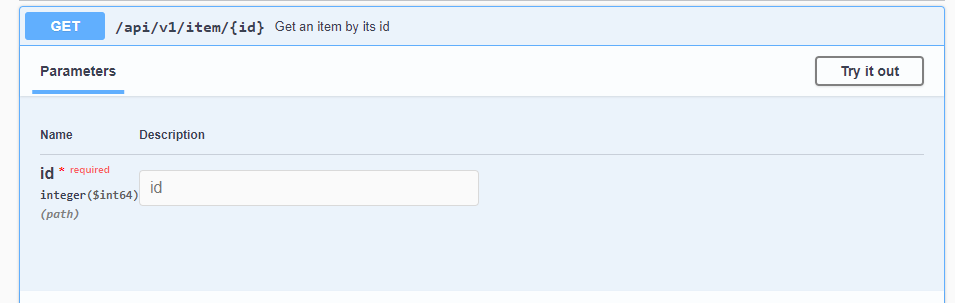
\includegraphics[width=\textwidth]{images/swagger-ui-execute.png}
    \caption{Using SwaggerUI to Execute \ac{API} requests}\label{img:swagger-execute}
\end{figure}

The generated specification can be used together with the web-based tool Swagger UI\footnote{\url{https://swagger.io/tools/swagger-ui/}}.
It can display the specification and the endpoints of the \ac{API} in a graphical format as shown in \autoref{img:swagger-explore}.
However, it can also be used to execute \ac{API} requests and display the result (see \autoref{img:swagger-execute}).
Swagger UI is included for every microservice of the case study and can be used as a graphical way to make requests to the \ac{API} for testing purposes.

\begin{figure}[!htb]
    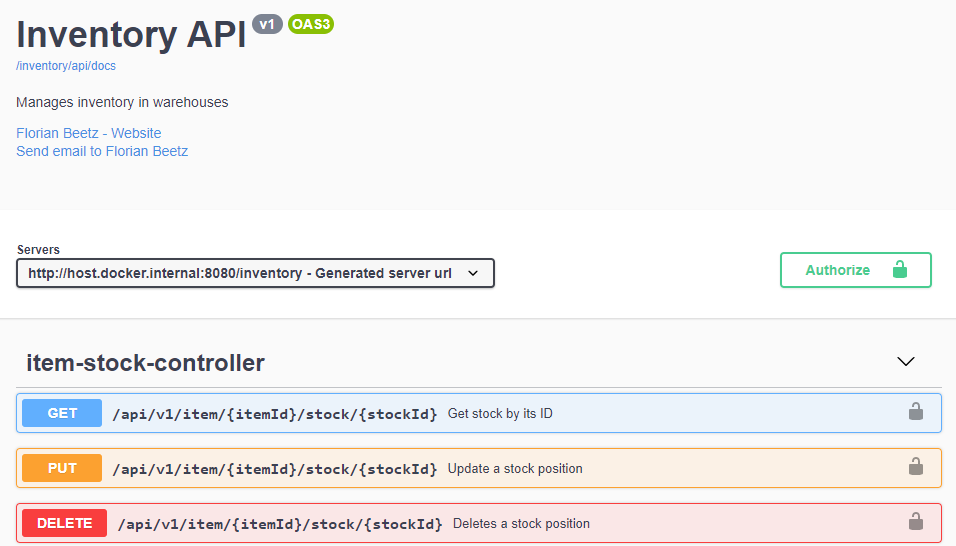
\includegraphics[width=\textwidth]{images/swagger-ui-explore.png}
    \caption{Using SwaggerUI to Explore \ac{API} endpoints}\label{img:swagger-explore}    
\end{figure}

\subsubsection{Client Authentication}

In order to implement a mechanism of authenticating users and checking if they are authorized to perform certain operations, \ac{OIDC} was used for the case study.
\ac{OIDC} is a common authentication and authorization scheme used in microservice architectures~\cite{Nehme2019, Hammann2020}.
In general, it can be used to implement \ac{SSO}, delegating authentication and obtaining user information from so-called \acp{IdP} such as Google or Microsoft.
This allows applications to rely on a user's identity provided by a trusted third-party, which is also the reason why these applications are called \acp{RP}.
The \acp{RP} never obtain the credentials of the user, only a token --- usually in the form of a \ac{JWT} --- is provided to them.
This token includes so called claims, which provide information about the authenticated user, and is signed with the private key of the \ac{IdP}.
Once, a token has been obtained by a \ac{RP}, its authenticity can be verified using the public key of the \ac{IdP}, thus \acp{RP} can be sure that the claims in the token have not been forged.
\autoref{lst:jwt-oidc} shows the payload of a \ac{JWT} by the \ac{IdP} of the \ac{REST} case study.
Each \ac{JSON} field in the payload represent a claim.
While some claims are standardized, in principle any claim can be included in a \ac{JWT}.
Lines one and two specify the expiration timestamp and issueing timestamp respectively.
The \texttt{iss} claim specifies the \ac{URL} of the issuing \ac{IdP} and \texttt{aud} specifies the intended audience of the token.
This information should be verified upon recieval of a token by the service to match the expected values.
The \texttt{Bearer} type specifies, that this token is intended to be sent using the \texttt{Bearer} scheme of \ac{HTTP} authentication.
Line six to eleven then contain the custom claims, first representing the roles the owner of the token has and their username.

\begin{lstlisting}[caption={\ac{JWT} Issued by an \ac{IdP}}, language=json, label={lst:jwt-oidc}]
{ "exp": 1605703187,
  "iat": 1605702887,
  "iss": "http://host.docker.internal:8080/auth/realms/ma-rest-shop",
  "aud": [ "shipping", "payment", "inventory", "order" ],
  "typ": "Bearer",
  "realm_access": {
    "roles": [ "payment_admin", "shipping_admin", "inventory_admin",
          "order_admin", "admin" ]
  },
  [...]
  "preferred_username": "admin"
}
\end{lstlisting}

Using \ac{OIDC} with a own \ac{IdP} makes \ac{OIDC} a suitable authentication mechanism for microservice architectures~\cite{Nehme2019}.
Because tokens and their claims can be verified locally at any service without relying on any external service, this authentication mechanism is easily scalable without introducing a bottleneck and without having to manage credentials locally for services.
The high-level architecture of the authentication mechanism of the case study is shown in \autoref{fig:oidc}.

\begin{figure}[!htb]
    \centering
    \begin{tikzpicture}[
    node distance=1cm,
    component/.style = {
        rectangle,
        draw,
        align = center,
        minimum height = 2cm,
        text width = 2cm
    },
    label/.style = {
        font=\footnotesize\sffamily
    }
]

\node[component] (ua) {Client};

\node[component, below right=of ua] (idp) {Identity Provider};

\node[component, below left= of ua] (svc2) {Service 2};
\node[component, left=of svc2] (svc1) {Service 1};

\draw[->] (ua.west) -| node[above, label, xshift=2cm] {\raisebox{.5pt}{\textcircled{\raisebox{-.9pt} {4}}} authenticated request} (svc1.north);

\draw[->] (ua.30) -| node[above, label, xshift=-1.3cm] {\raisebox{.5pt}{\textcircled{\raisebox{-.9pt} {2}}} authentication} (idp.50);
\draw[->] (idp.130) |- node[above, label, xshift=0.2cm] {\raisebox{.5pt}{\textcircled{\raisebox{-.9pt} {3}}} signed token} (ua.330);

\draw[->] (ua.270) |- node[below, label, text width=3cm, xshift=-0.2cm] {\raisebox{.5pt}{\textcircled{\raisebox{-.9pt} {5}}} authenticated request} (svc2.0);

\draw[->] (svc1.270) -- +(0,-5mm) -| node[below, label, xshift=-5cm] {\raisebox{.5pt}{\textcircled{\raisebox{-.9pt} {1}}} obtain public key} (idp.270);
\draw (svc2.south) -- +(0,-5mm);
\end{tikzpicture}
    \caption{\ac{OIDC} in a Microservice Architecture}\label{fig:oidc}
\end{figure}

First, each service obtains the public key of the \ac{IdP} at startup for token verification.
Then, whenever a client wants to send a request to any service, the user provides their credentials to the \ac{IdP} and obtains a signed token.
Lastly, the obtained token can be used to send authenticated requests to any service.
The services verify the authenticitiy of the token using the obtained public key of the first step.
If the signature of the token is valid, the services can trust the user to have the roles as claimed in the token.

\begin{table}[!htb]
    \centering
    \begin{tabular}{@{}lcccc@{}}
        \toprule
        \multirow{2}{*}{\textbf{Role}}  & \multicolumn{4}{c}{\textbf{Service Accounts}} \\
                                        & Inventory & Order & Payment   & Shipping      \\
        \midrule
        \texttt{inventory\_admin}       & ---       & x     &           & x             \\
        \texttt{order\_admin}           &           & ---   & x         & x             \\
        \texttt{payment\_admin}         &           & x     & ---       &               \\
        \texttt{shipping\_admin}        &           & x     &           & ---           \\
        \bottomrule
        
    \end{tabular}
    \caption{Available Roles for the \ac{REST} Case Study and Service Account Association}\label{tab:roles-rest}
\end{table}


\begin{itemize}
    \item OIDC via Keycloak
    \item explain how OIDC works and why it is a good choice for microservices
    \item Service-to-Service communication is also authenticated via Service Accounts
\end{itemize}

\subsubsection{Service-to-Service Communication}

\begin{itemize}
    \item Code-generation for OpenAPI specifications are available
    \item Clients were implemented by hand because of the higher control and because Spring provides an automated mechanism to authenticate client requests
    \item Different clients for each service, scoped to the required functionality
\end{itemize}

\subsubsection{Optimistic Locking for Write-Operations using \acs{HTTP}}

When using \ac{REST} with the stateless protocol \ac{HTTP}, the problem of handling concurrent modifications to a resource arises.
When users try to update a resource at the same time, the update of the first user is overwritten.
This problem is shown in \autoref{fig:lost-update}, where two clients send \ac{HTTP} \texttt{PUT} requests to the same resource.
The server processes the first update and returns a response indicating that the resource was successfully updated.
Meanwhile, an update request of the second client is received and the changes of the other client are overwritten.

\begin{figure}[!htb]
    \centering
    \begin{tikzpicture}[
    node distance=4cm,
    instance/.style = {
        draw,
        minimum height = 1.5\baselineskip,
        thick
    },
    lifeline/.style = {
        dotted,
        thick
    },
    packet/.style = {
        above,
        yshift=0.25cm,
        font=\ttfamily
    }
]

\node[instance] (c1) {:Client};
\node[instance, right=of c1] (server) {:Server};
\node[instance, right=of server] (c2) {:Client};

\draw[lifeline] (c1.south) -- + (0,-5);
\draw[lifeline] (server.south) -- + (0,-5);
\draw[lifeline] (c2.south) -- + (0,-5);

\draw[->] ($(c1.south)-(0,0.5)$) -- node[packet] {PUT /item/1 HTTP/1.1} ($(server.south)-(0,1.5)$);
\draw[->] ($(c2.south)-(0,1)$) -- node[packet] {PUT /item/1 HTTP/1.1} ($(server.south)-(0,2)$);

\draw[->] ($(server.south)-(0,3)$) -- node[packet] {HTTP/1.1 200 OK} ($(c1.south)-(0,4)$);
\draw[->] ($(server.south)-(0,3.5)$) -- node[packet] {HTTP/1.1 200 OK} ($(c2.south)-(0,4.5)$);

\end{tikzpicture}
    \caption{Lost Update Problem}\label{fig:lost-update}
\end{figure}

To solve this problem, a locking mechanism needs to be implemented.
However, both \ac{HTTP} and \ac{REST} mandate statelessness of the communication.
Thus, an optimistic locking procedure must be implemented to comply with these restrictions.
\ac{HTTP} provides several ways of implementing optimistic locking procedures using so-called conditional requests~\cite{MDN2020}.
Conditional requests include a condition that is evaluated by the server and only if this condition holds, the request is executed.
This kind of request is realized with the \ac{HTTP} headers \texttt{If-Match} or \texttt{If-None-Match} that indicate that the requested resource should have or respectively not have a specified hash value provided by the server using the \texttt{ETag} (Entity Tag) header.
Alternatively, \texttt{If-Modified-Since} or \texttt{If-Unmodified-Since} can be used, to indicate that the request should only be executed if the resource was or was not modified since a given point in time.

For the case study, the approach of implementing locking using \texttt{ETag}s and sending requests with \texttt{If-Match} was implemented because the time based conditional requests only be support a granularity of seconds.
If multiple requests are made within the same second, the lost update problem still persists.
\autoref{lst:locking-response} shows the response to a \texttt{GET} request to an updatable resource.
Notably, the response contains an \texttt{ETag} header.

\begin{lstlisting}[caption={Response to \texttt{GET} Requests for Updatable Resources}, showlines=true, label=lst:locking-response, language=http]
[*HTTP/1.1 200 OK*]
Content-Type: application/json
(*\textit{\textbf{ETag}: 12345}*)

{"title": "Item", "price": 1.99}
\end{lstlisting}

If this resource is to be updated, \texttt{PUT} requests must include the \texttt{If-Match} header as shwon in \autoref{lst:locking-request}.
Otherwise, the server will respond with the \texttt{428 Precondition Required} status and not execute the request.
Only if the provided entity tag matches the resource currently stored at the server, the request is updated.
Whenever the entity tag does not match, the server responds with the status code \texttt{412 Precondition Failed}.

\begin{lstlisting}[caption={Request to Update Resources}, showlines=true, label=lst:locking-request, language=http]
[*PUT /item/1 HTTP/1.1*]
Content-Type: application/json
(*\textit{\textbf{If-Match}: 12345}*)

{"title": "Item", "price": 2.49}
\end{lstlisting}

\subsection{Implementation of GraphQL Microservices}

\subsubsection{Technology Stack}

Similar to the \ac{REST} implementation of the microservices, Java and the Spring framework were used for the GraphQL microservices.
To implement the GraphQL interfaces, third-party modules for the Spring framework were used.
The \textit{GraphQL Spring Boot Starter}\footnote{\url{https://github.com/graphql-java-kickstart/graphql-spring-boot}} automatically configures an GraphQL endpoint and sets up GraphiQL.% checktex 13
Federating the schemas of the microservices is achived using the \textit{Appollo Federation on the \acs{JVM}}\footnote{\url{https://github.com/apollographql/federation-jvm}} module.

The individual microservices are packaged as Docker Linux containers and a Traefik reverse proxy is placed before the network interfaces of the containers.
Each of the services provides its own GraphQL endpoint that can process queries requesting objects the service owns, e.g.~the inventory service can process queries about items and where they are stored.
However, to be able to query data from multiple services in one request, a federation gateway is needed.
This allows for example to query the names of all items in an order, where the order microservice and the inventory microservice would be involved.
The gateway is implemented as a Node.js application using the Apollo stack\footnote{\url{https://www.apollographql.com/}}.

\begin{figure}[!htb]
    \centering
    \begin{tikzpicture}[
    node distance=1.25cm,
    container/.style = {
        draw
    },
    application/.style = {
        draw,
        regular polygon,
        regular polygon sides = 4,
        text width=.5cm,
        align = center
    },
    database/.style = {
        draw,
        cylinder,
        shape border rotate=90,
        aspect=0.25,
        text width = .5cm,
        minimum height = 1cm,
        align = center%,
        %cylinder uses custom fill, cylinder body fill=white, cylinder end fill=black!5
    },
]

\node[application, color=theme5, fill=theme5!10!white, below=1.5cm of traefik] (order1) {O};
\node[application, color=theme5, fill=theme5!10!white, left=of order1] (order2) {O};
\node[application, color=theme3, fill=theme3!10!white, left=of order2] (inventory) {I};
\node[application, color=theme1, fill=theme1!10!white, right=of order1] (payment) {P};
\node[application, color=theme2, fill=theme2!10!white, right=of payment] (shipping) {S};

\draw ($(inventory.north west) + (-1cm,1.25cm)$) -- ($(shipping.north east) + (2cm,1.25cm)$)
    -- +(0,5cm) -- ($(inventory.north west) + (-1cm,6.25cm)$) -- +(0,-1cm) -- ($(shipping.north east) + (1cm, 5.25cm)$)
    -- +(0,-3cm) -- ($(inventory.north west) + (-1cm, 2.25cm)$) -- cycle;
\node[rotate=90] at ($(shipping.north east) + (1.5cm, 3.75cm)$) {
\includegraphics[width=.5cm,page=1]{images/image.pdf} Reverse Proxy};

\draw ($(inventory.north west) + (-0.5cm,2.75cm)$) -- +(0,2cm) -- ($(shipping.north east) + (0.5cm,4.75cm)$) -- +(0,-2cm) -- cycle;

\draw[->] ($(inventory.north) + (0,1.25cm)$) -- (inventory);
\draw[->] ($(order1.north) + (0,1.25cm)$) -- (order1);
\draw[->] ($(order2.north) + (0,1.25cm)$) -- (order2);
\draw[->] ($(payment.north) + (0,1.25cm)$) -- (payment);
\draw[->] ($(shipping.north) + (0,1.25cm)$) -- (shipping);

\coordinate (gwCenter) at ($(inventory.north west)!0.5!(shipping.north east) + (0cm,3.75cm)$);
\coordinate (oCenter) at ($(order1.north)!0.5!(order2.north)$);

\node[rotate=90] at ($(gwCenter)+(-5.25cm,0)$) {Gateway};

\draw ($(inventory.north west)!0.5!(shipping.north east) + (0,7.25cm)$) -- node[above,yshift=.25cm,text width=5cm,align=center] {\acs{HTTP} requests\\(external and internal)} +(0,-1cm);
\draw[dashed] ($(inventory.north west)!0.5!(shipping.north east) + (0,6.25cm)$) -- node[right] {\footnotesize\texttt{/gateway/*}} +(0,-1cm);
\draw[->] ($(gwCenter) + (0,1.5cm)$) -- +(0,-0.5cm);
\draw[dashed] ($(gwCenter) + (0,1cm)$) -- +(0,-1cm) -| ($(inventory.north)+(0,2.75cm)$);
\draw[dashed] (gwCenter) -| ($(shipping.north)+(0,2.75cm)$);
\draw[dashed] ($(payment.north)+(0,2.75cm)$) -- +(0,1cm);
\draw[dashed] ($(oCenter)+(0,2.75cm)$) -- +(0,1cm);

\draw[->] ($(inventory.north)+(0,2.75cm)$) -- +(0,-0.5cm);
\draw[->] ($(shipping.north)+(0,2.75cm)$) -- +(0,-0.5cm);
\draw[->] ($(payment.north)+(0,2.75cm)$) -- +(0,-0.5cm);
\draw[->] ($(oCenter)+(0,2.75cm)$) -- +(0,-0.5cm);

\draw[dashed] ($(inventory.north) + (0,1.25cm)$) -- node[right] {\footnotesize\texttt{/inventory/*}} +(0,1cm);
\draw[dashed] ($(order1.north) + (0,1.25cm)$) -- +(0,0.5cm) -| node[right,xshift=1.2cm] {\footnotesize\texttt{/order/*}} ($(oCenter)+(0,2.25cm)$);
\draw[dashed] ($(oCenter)+(0,1.75cm)$) -| ($(order2.north) + (0,1.25cm)$);
\draw[dashed] ($(payment.north) + (0,1.25cm)$) -- node[right] {\footnotesize\texttt{/payment/*}} +(0,1cm);
\draw[dashed] ($(shipping.north) + (0,1.25cm)$) -- node[right] {\footnotesize\texttt{/shipping/*}} +(0,1cm);

\node[database, color=theme3, fill=theme3!10!white, below=of inventory] (invDb) {};
\node[database, color=theme1, fill=theme1!10!white, below=of payment] (payDb) {};
\node[database, color=theme2, fill=theme2!10!white, below=of shipping] (shipDb) {};
\node[database, color=theme5, fill=theme5!10!white, below=of $(order1.south)!0.5!(order2.south)$] (ordDb) {};

\draw[->] (inventory) -- (invDb);
\draw[->] (order1) |- (ordDb);
\draw[->] (order2) |- (ordDb);
\draw[->] (payment) -- (payDb);
\draw[->] (shipping) -- (shipDb);

\end{tikzpicture}
    \caption{Containers for the GraphQL Microservice Architecture}\label{fig:graphql-containers}
\end{figure}

\autoref{fig:graphql-containers} shows the same deployment with two deployed order microservices for the GraphQL implementation.
The gateway and the reverse proxy are intertwined because both the gateway and the microservices should be able to be scaled horizontally.
This requires that the external requests to the gateway, the requests of the gateway to the microservices, and the requests of the microservices to the gateway are all routed through the reverse proxy.

\subsubsection{\acs{API} Style}

\begin{enumerate}
    \item API exposes a single endpoint where all requests are made to
    \item API has more of a resource-API for queries but is completely RPC-based for mutations
    \item Entities are identified by an ID that they expose to clients
\end{enumerate}

\subsubsection{GraphQL Federation Gateway}

\begin{lstlisting}[caption={Schema Definition to Enable Federation}, language=graphqls]
type Item @key(fields: "id") {
    # [...]
}
\end{lstlisting}

\begin{lstlisting}[caption={Implementation of the GraphQL Gateway}, language=javascript]
const gateway = new ApolloGateway({
    serviceList: [
        { name: 'inventory', url: inventoryHost },
        // [...]
    ]
});
const server = new ApolloServer({ gateway });
server.listen();
\end{lstlisting}

\begin{itemize}
    \item Federation allows multiple schemas to be combined to one big one
    \item Individual schemas expose extra information on what additional information a service can provide to an object it does not own and how to identify objects of services it does not own
    \item A gateway is required to combine the schemas, generate query plans upon requests and dispatch sub-queries to the services
\end{itemize}

\subsubsection{Data Fetching}

\begin{lstlisting}[caption={Data Fetching in \acs{API} Models}, language=java]
public class Item {
    private final long id; // [...]
    private final Supplier<Long> totalInStockSupplier;

    public Item(long id, // [...]
                Supplier<Long> totalInStockSupplier) {
        this.id = id; // [...]
        this.totalInStockSupplier = totalInStockSupplier;
    }
    // [...]
    public List<ItemStock> getStock(Integer page, Integer size) {
        return itemStockSupplier.apply(page, size);
    }
}
\end{lstlisting}

\begin{lstlisting}[caption={\acs{API} Model Creation with Fetcher Injection}, language=java]
public class ItemService {
    @Autowired private ItemRepository itemRepository;
    @Autowired private ItemStockService itemStockService;
    // [...]
    public Item lookupItem(long id) {
        return itemRepository.findById(id)
                             .map(this::fromEntity)
                             .orElse(null);
    }
    // [...]
    Item fromEntity(ItemEntity entity) {
        return new Item(
                entity.getId(), // [...]
                () -> itemStockService.lookupTotalInStock(entity.getId())
        );
    }
    // [...]
}
\end{lstlisting}

\begin{itemize}
    \item Complex data fetching, because responses are highly customizable by the user
    \item Data fetching needs to respect eventualities without requesting large amounts of data from the database that the user did not request
\end{itemize}

\subsubsection{GraphiQL and GraphQL Playground}

\begin{itemize}
    \item GraphiQL is a simple web editor for GraphQL queries
    \item GraphQL Playground is more advanced and is used at the gateway
\end{itemize}

\subsubsection{Client Authentication}

\begin{itemize}
    \item Also OICD using Keycloak was used
    \item Authentication can be done on a much granular level -> some clients are not allowed to read certain fields of an entity
\end{itemize}

\subsubsection{Service-to-Service communication}

\begin{itemize}
    \item Code for serializing requests and parsing responses was generated
    \item Transport mechanism was intentionally done by hand, as it allows to easily inject authentication
    \item Means to generate full clients exist
\end{itemize}

\subsection{Architectural Differences of the Implementations}

\subsubsection{\acs{HTTP} Interface}

GraphQL only has one single endpoint, whereas REST specifies the action to execute through an endpoint.

\subsubsection{\acs{API} Paradigms}

REST implementation hides the fact that a complex, service-spanning operation is triggered upon status updates.
A generic request is made to update a resource for REST, whereas GraphQL makes it explicit, that an action is to be executed on the server.

\subsubsection{Authentication and Authorization}

Authentication is the same, authorization can be easily implemented on a very granular level.
Implementing the same for REST is possible, but requires much more effort.

\subsection{Performance Comparison}

\textbf{To do}

\subsection{Schema Evolution}

\textbf{To do}

\subsection{Discussion}

\textbf{To do}